\documentclass[11pt,a4paper]{article}

\usepackage[margin=2.2cm]{geometry}
\usepackage[T1]{fontenc}
\usepackage{lmodern}
\usepackage{amssymb}
\usepackage{xcolor}
\usepackage{tikz}
\usetikzlibrary{arrows.meta,positioning}
\usepackage{booktabs}
\usepackage{tabularx}
\usepackage{enumitem}
\usepackage{listings}
\usepackage[most]{tcolorbox}
\usepackage{fancyhdr}
\usepackage[colorlinks=true,linkcolor=blue!50!black,urlcolor=blue!50!black]{hyperref}

\definecolor{local}{HTML}{2E7D32}
\definecolor{cloud}{HTML}{1565C0}
\definecolor{warn}{HTML}{C62828}
\definecolor{idea}{HTML}{6A1B9A}
\definecolor{soft}{HTML}{F5F5F5}

\newtcolorbox{concept}[1]{colback=idea!4,colframe=idea!70,fonttitle=\bfseries,title={Concept: #1},breakable}
\newtcolorbox{analogy}{colback=local!5,colframe=local!70,fonttitle=\bfseries,title={Analogy},breakable}
\newtcolorbox{why}{colback=cloud!4,colframe=cloud!70,fonttitle=\bfseries,title={Why it is done this way},breakable}
\newtcolorbox{caution}{colback=warn!4,colframe=warn!70,fonttitle=\bfseries,title={Watch out},breakable}
\newtcolorbox{exercise}{colback=soft,colframe=black!50,fonttitle=\bfseries,title={Check yourself},breakable}

\lstset{basicstyle=\ttfamily\small,backgroundcolor=\color{soft},frame=single,
        rulecolor=\color{black!25},columns=fullflexible,keepspaces=true,
        showstringspaces=false,breaklines=true}

\pagestyle{fancy}
\fancyhf{}
\lhead{\small Listen -- Learning Doc 03}
\rhead{\small Commands and the Intent Engine}
\cfoot{\thepage}

\title{\textbf{Listen}\\[4pt]\large Learning Doc 03: Commands and the Intent Engine\\
       \normalsize How ``search what is an atom'' becomes an action}
\author{Detailed design, Section 2}
\date{7 October 2026}

\begin{document}
\maketitle

\begin{abstract}
\noindent The voice module hands us a line of text, such as \texttt{"search what is an atom"}.
This document designs everything between that text and an action on your screen: the file
format that describes commands, the matching algorithm that picks the right command, how
default apps work, how you add and edit commands without code, and why the design is safe even
when an AI writes the commands. Each new idea is introduced as a concept box.
\end{abstract}

\tableofcontents
\newpage

% =====================================================================
\section{The problem in one picture}

\begin{center}
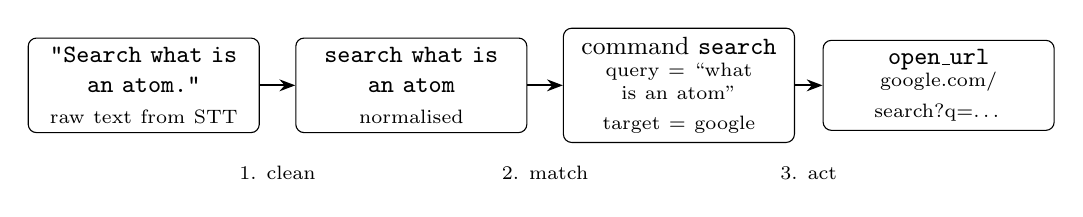
\begin{tikzpicture}[font=\small,
  st/.style={draw,rounded corners=3pt,align=center,minimum height=1.1cm,text width=2.7cm,fill=white},
  arr/.style={-{Stealth[length=2mm]},thick}]
\node[st] (a) {\texttt{"Search what is\\an atom."}\\\scriptsize raw text from STT};
\node[st,right=0.45cm of a] (b) {\texttt{search what is\\an atom}\\\scriptsize normalised};
\node[st,right=0.45cm of b] (c) {command \texttt{search}\\\scriptsize query = ``what is an atom''\\\scriptsize target = google};
\node[st,right=0.35cm of c] (d) {\texttt{open\_url}\\\scriptsize google.com/\\\scriptsize search?q=\ldots};
\draw[arr] (a) -- node[below,font=\scriptsize,yshift=-9mm]{1. clean} (b);
\draw[arr] (b) -- node[below,font=\scriptsize,yshift=-9mm]{2. match} (c);
\draw[arr] (c) -- node[below,font=\scriptsize,yshift=-9mm]{3. act} (d);
\end{tikzpicture}
\end{center}

\noindent Three steps: \textbf{clean} the text, \textbf{match} it to a command and pull out the
interesting parts, then \textbf{act}. This document covers steps 1 and 2 in detail, and the
contract between step 2 and step 3.

\begin{concept}{Intent and slots}
An \textbf{intent} is \emph{what you want done} (``search''). \textbf{Slots} are the
\emph{details} needed to do it (the query ``what is an atom'', the target ``google'').
Turning a sentence into an intent plus filled slots is called \textbf{intent parsing} or
\textbf{slot filling}. Siri, Alexa and Google Assistant all have this exact step.
\end{concept}

% =====================================================================
\section{The command file}

\subsection{Data-driven design}
\begin{concept}{Data-driven design}
Instead of writing behaviour as code (\texttt{if text.startswith("search")}\ldots), you
describe behaviour in a \textbf{data file}, and write one small, general piece of code that
reads the file and follows it. Changing behaviour means editing data, not code.
\end{concept}

This is what makes your requirement ``add \texttt{play \{query\} on spotify} without touching
code'' possible. The file is written in \textbf{YAML}, a format designed to be easy for humans to
read and edit: indentation shows nesting, \texttt{-} starts a list item, \texttt{key: value} sets
a field.

\subsection{Three sections: targets, defaults, commands}

\begin{lstlisting}
version: 1

# targets: the places Listen can send you
targets:
  google:  { search: "https://www.google.com/search?q={query}",
             home:   "https://www.google.com" }
  youtube: { play:   "https://www.youtube.com/results?search_query={query}",
             search: "https://www.youtube.com/results?search_query={query}",
             home:   "https://www.youtube.com" }
  spotify: { play:   "https://open.spotify.com/search/{query}",
             home:   "https://open.spotify.com" }

# defaults: which target a verb uses when you don't name one
defaults:
  search: google
  play:   youtube

# commands: sentence patterns -> an action primitive
commands:
  - id: search
    patterns: ["search {query} on {target}", "search {query}",
               "look up {query}", "google {query}"]
    action: open_url
    url_from: search          # use the target's "search" URL

  - id: play
    patterns: ["play {query} on {target}", "play {query}"]
    action: open_url
    url_from: play

  - id: open
    patterns: ["open {app}", "launch {app}", "start {app}"]
    action: launch_app

  - id: close
    patterns: ["close {app}", "quit {app}", "exit {app}"]
    action: close_app

  - id: volume_set
    patterns: ["volume {number}", "set volume to {number}"]
    action: set_volume
  - id: volume_up
    patterns: ["volume up", "louder", "turn it up"]
    action: change_volume
    params: { step: 10 }
  - id: volume_down
    patterns: ["volume down", "quieter", "turn it down"]
    action: change_volume
    params: { step: -10 }
  - id: mute
    patterns: ["mute", "unmute"]
    action: toggle_mute
\end{lstlisting}

\begin{why}
\textbf{Targets} are separated from \textbf{commands} because ``where'' and ``what'' change for
different reasons (the single-responsibility idea from Doc~02). Look at what this buys you:
\texttt{play \{query\} on spotify} needs \emph{no new command at all}. The \texttt{play} command
already accepts \texttt{on \{target\}}; you only add a \texttt{spotify} target with a
\texttt{play} URL. One new line of data, and \emph{every} verb that has a URL for Spotify
starts working with it.
\end{why}

\subsection{Slot types}
Every \texttt{\{name\}} in a pattern is a slot, and its name decides what it may contain:

\begin{center}
\renewcommand{\arraystretch}{1.2}
\begin{tabularx}{\textwidth}{l X l}
\toprule
\textbf{Slot} & \textbf{Accepts} & \textbf{Example} \\
\midrule
\texttt{\{query\}}  & Any text (at least one word) & ``what is an atom'' \\
\texttt{\{target\}} & Only names in \texttt{targets} & ``spotify'' \\
\texttt{\{app\}}    & An app Listen can find on your PC (Section~\ref{sec:apps}) & ``vs code'' \\
\texttt{\{number\}} & A number, written as digits or words & ``50'', ``fifty'' \\
\bottomrule
\end{tabularx}
\end{center}

\noindent Typed slots are how the matcher tells ``play \emph{songs on the beach}'' (the
\emph{query} is ``songs on the beach'', because ``the beach'' is not a target) apart from
``play \emph{lofi} on \emph{spotify}''.

% =====================================================================
\section{Step 1: normalisation}

\begin{concept}{Normalisation}
Different-looking inputs that mean the same thing are converted into one standard form
\emph{before} comparing them. ``Search what is an atom.'', ``search what is an atom'' and
``SEARCH what is an atom?'' must all match the same pattern.
\end{concept}

\noindent The cleaner, in order:
\begin{enumerate}[nosep]
  \item Lowercase everything.
  \item Remove punctuation the speech engine adds (\texttt{. , ? !}), but keep characters
        that matter inside queries such as \texttt{+} and \texttt{'} in ``what's''.
  \item Remove the wake word if it leaked into the transcript (``hey jarvis search\ldots'').
  \item Remove polite filler at the start and end: ``please'', ``can you'', ``could you'',
        ``for me''. (``Can you please search atoms for me'' $\to$ ``search atoms''.)
  \item Collapse repeated spaces.
\end{enumerate}

% =====================================================================
\section{Step 2: matching}

\subsection{Patterns become regular expressions}
\begin{concept}{Regular expression (regex)}
A \textbf{regex} is a tiny language for describing text patterns. For example
\texttt{\^{}search (?P<query>.+)\$} means: the text \emph{starts} (\texttt{\^{}}) with
``search '', then one or more characters (\texttt{.+}) that we capture under the name
\texttt{query}, then the text \emph{ends} (\texttt{\$}). Python's built-in \texttt{re} module
runs them.
\end{concept}

You never write regexes yourself. When the command file loads, each friendly pattern is
\emph{compiled} into one:

\begin{center}
\renewcommand{\arraystretch}{1.2}
\begin{tabularx}{\textwidth}{l X}
\toprule
\textbf{Pattern in YAML} & \textbf{Regex the engine builds} \\
\midrule
\texttt{search \{query\}} & \texttt{\^{}search (?P<query>.+?)\$} \\
\texttt{play \{query\} on \{target\}} & \texttt{\^{}play (?P<query>.+?) on (?P<target>.+?)\$} \\
\bottomrule
\end{tabularx}
\end{center}

\noindent The \texttt{\^{}} and \texttt{\$} \emph{anchors} mean the whole sentence must fit
the pattern, so ``research papers'' does not accidentally match ``search \{query\}''.

\subsection{When several patterns match: specificity}
``play lofi on spotify'' matches \emph{both}
\begin{itemize}[nosep]
  \item \texttt{play \{query\} on \{target\}} with query = ``lofi'', target = ``spotify'', and
  \item \texttt{play \{query\}} with query = ``lofi on spotify''.
\end{itemize}

\begin{concept}{Specificity}
When several rules match, prefer the \textbf{most specific} one: the one that explains more of
the sentence with fixed words. Score = number of literal words in the pattern. The first
pattern has 2 (``play'', ``on''); the second has 1. The first wins. On a tie, the command
listed earlier in the file wins, so the order of the file is a tiebreaker you control.
\end{concept}

\subsection{Validation can reject a match}
After a regex matches, each slot is checked against its type. If a check fails, \emph{that
candidate is thrown away} and the next-best one is tried:

\begin{lstlisting}
"play songs on the beach"
  candidate 1: play {query} on {target}  target="the beach" -> not a target, REJECT
  candidate 2: play {query}              query="songs on the beach"  -> ACCEPT
\end{lstlisting}

\subsection{Defaults fill missing slots}
If the winning pattern has no \texttt{\{target\}} (``play lofi''), the engine looks up
\texttt{defaults.play} $\to$ \texttt{youtube}. If the target has no URL for that verb (asking
Google to ``play'' something), the result is a clear error message instead of a guess.

\subsection{No match is useful information}
If nothing matches, the engine publishes an \texttt{IntentNotMatched} event. The terminal says
``Sorry, I didn't understand: \ldots'', and the sentence is logged. Later, your analytics page
can list \emph{what you tried that failed}: exactly the commands worth adding next.

\subsection{The whole algorithm}
\begin{lstlisting}
match(text):
    text = normalise(text)
    candidates = []
    for each command, for each pattern:
        if pattern.regex fully matches text:
            slots = the captured groups
            if every slot passes its type check:
                candidates.append( (specificity, file_order, command, slots) )
    if no candidates: return NoMatch(text)
    best = highest specificity, then earliest in file
    fill missing target from defaults
    return Intent(command, slots)
\end{lstlisting}

\begin{why}
This is a \textbf{pure function}: text in, result out, no microphone, no files, no internet,
no side effects. That makes it trivial to test with a table of example sentences, and it runs
in well under a millisecond, so matching costs nothing on your lightweight budget.
\end{why}

% =====================================================================
\section{Finding apps by name}\label{sec:apps}

``open vs code'' requires knowing that ``vs code'' means
\texttt{C:\textbackslash...\textbackslash Code.exe}. Windows already keeps that knowledge: every
installed app puts a \textbf{shortcut} in the Start Menu folders.

\begin{enumerate}[nosep]
  \item At startup the agent scans the Start Menu shortcut folders and builds an
        \textbf{app index}: display name $\to$ how to launch it. This takes a fraction of a
        second and is refreshed when you ask (``refresh apps'') or once a day.
  \item You can add \textbf{aliases} in the command file (\texttt{"code": "Visual Studio
        Code"}) for names the speech engine spells oddly.
  \item The \texttt{\{app\}} slot is matched with \textbf{fuzzy matching}.
\end{enumerate}

\begin{concept}{Fuzzy matching}
Exact comparison fails on ``vs code'' vs.\ ``Visual Studio Code'' or ``spotfy'' vs.\
``Spotify''. Fuzzy matching gives a \textbf{similarity score} between 0 and 1 and accepts the
best candidate above a threshold (we start at 0.8 and tune it). Python's built-in
\texttt{difflib} does this with no extra download.
\end{concept}

\noindent ``open google'' works too: if the name is not an app but \emph{is} a target, Listen
opens that target's \texttt{home} URL.

% =====================================================================
\section{Step 3: the contract with the action executor}

The intent engine never performs actions itself. It publishes an \texttt{IntentMatched} event:

\begin{lstlisting}
IntentMatched(
    command_id = "search",
    action     = "open_url",
    args       = { "url": "https://www.google.com/search?q=what+is+an+atom" },
    heard      = "search what is an atom",
)
\end{lstlisting}

\noindent The \texttt{actions/} module subscribes and runs it. Values placed into URLs are
\textbf{URL-encoded} (spaces become \texttt{+}, \texttt{\&} becomes \texttt{\%26}), so a
query can never break the URL or sneak in extra parameters.

\subsection{The v1 action primitives}
\begin{center}
\renewcommand{\arraystretch}{1.2}
\begin{tabularx}{\textwidth}{l X}
\toprule
\textbf{Primitive} & \textbf{What it does} \\
\midrule
\texttt{open\_url}      & Opens a web address in your default browser \\
\texttt{launch\_app}    & Starts an app from the app index \\
\texttt{close\_app}     & Asks an app's windows to close (like clicking X, so unsaved-work prompts still appear) \\
\texttt{set\_volume}    & Sets master volume to 0--100 \\
\texttt{change\_volume} & Raises or lowers volume by a step \\
\texttt{toggle\_mute}   & Mutes or unmutes \\
\bottomrule
\end{tabularx}
\end{center}

\begin{caution}
\textbf{Honest limitation:} \texttt{play lofi} opens YouTube's \emph{search results} for
``lofi''; it does not start the first video automatically. Autoplay would need either the
YouTube API or scraping the results page. It is a possible later improvement, deliberately out
of v1.
\end{caution}

% =====================================================================
\section{Adding and editing commands without code}

\subsection{Where the file lives}
\begin{itemize}[nosep]
  \item A \textbf{default} command file ships inside the agent's code (versioned in git).
  \item On first run it is copied to your user-data folder
        (\texttt{\%APPDATA\%\textbackslash Listen\textbackslash commands.yaml}). That copy is
        yours: edits go there, and code updates never overwrite it.
  \item Once sync exists (Section 5 of the design), the cloud holds the master copy, so edits
        made in the web app reach your laptop.
\end{itemize}

\subsection{Validation on every load}
\begin{concept}{Schema validation}
A \textbf{schema} is a machine-checkable description of what valid data looks like:
``every command must have an \texttt{id}, at least one pattern, and an \texttt{action} that is
one of the six primitives''. Before using the file, the agent checks it against
\texttt{shared/recipe.schema.json} (the contract from Doc~02).
\end{concept}

\noindent An invalid entry is \textbf{skipped with a clear warning}, and every valid entry still
loads. One typo never takes down the whole assistant.

\subsection{The command builder}
\begin{center}
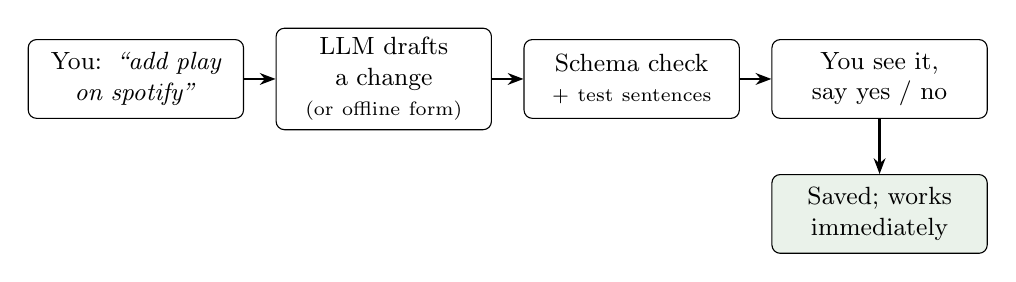
\begin{tikzpicture}[font=\small,
  st/.style={draw,rounded corners=3pt,align=center,minimum height=1cm,text width=2.5cm,fill=white},
  arr/.style={-{Stealth[length=2mm]},thick}]
\node[st] (a) {You: \emph{``add play on spotify''}};
\node[st,right=0.4cm of a] (b) {LLM drafts a change\\\scriptsize (or offline form)};
\node[st,right=0.4cm of b] (c) {Schema check\\\scriptsize + test sentences};
\node[st,right=0.4cm of c] (d) {You see it,\\say yes / no};
\node[st,below=0.7cm of d,fill=local!10] (e) {Saved; works\\immediately};
\draw[arr] (a)--(b); \draw[arr] (b)--(c); \draw[arr] (c)--(d); \draw[arr] (d)--(e);
\end{tikzpicture}
\end{center}

\begin{enumerate}[nosep]
  \item You describe the change in plain words: add a target, add a command, change a default,
        add a pattern, rename or delete something.
  \item The LLM receives your request, the current file, and the schema, and returns a
        \emph{proposed change} (not a rewritten file).
  \item The proposal is validated against the schema and tried on a few example sentences
        (``play lofi on spotify'' should now match).
  \item You see a readable diff and approve or reject it. Nothing is saved before ``yes''.
\end{enumerate}

\noindent Offline, a guided form asks the same questions step by step.

\subsection{Why this is safe}
\begin{concept}{Allowlist}
An \textbf{allowlist} is a fixed list of things that are permitted; everything else is
refused. Listen's six primitives are an allowlist. A command can only ever \emph{combine}
them; there is deliberately \textbf{no} ``run any program with any arguments'' primitive.
\end{concept}

\begin{why}
An AI is writing data that your computer will act on, so you must ask: what is the worst a
bad (or tricked) suggestion could do? With the allowlist, the worst case is ``opens a wrong
website'' or ``closes an app politely''. Without it, the worst case is ``runs any command on
your PC''. Combined with your approval step and URL encoding, this keeps the AI helpful but
harmless. Good design limits damage \emph{structurally}, rather than hoping nothing goes wrong.
\end{why}

% =====================================================================
\section{Testing this design}
The matcher is a pure function, so its tests are a simple table:

\begin{lstlisting}
"search what is an atom"            -> search, query="what is an atom", target=google
"Can you search atoms please?"      -> search, query="atoms"
"play lofi"                         -> play,   query="lofi",  target=youtube
"play lofi on spotify"              -> play,   query="lofi",  target=spotify
"play songs on the beach"           -> play,   query="songs on the beach", target=youtube
"volume fifty"                      -> volume_set, number=50
"research papers"                   -> no match
"open vs code"                      -> open,   app="Visual Studio Code"
\end{lstlisting}

\noindent Every bug we ever find in matching becomes one more row in this table, so it can never
come back unnoticed. That habit is called a \textbf{regression test}.

% =====================================================================
\section{Glossary}
\begin{description}[style=nextline,leftmargin=1.2cm,itemsep=2pt]
  \item[Allowlist] A fixed list of permitted things; everything else is refused.
  \item[Anchors] Regex symbols \texttt{\^{}} (start) and \texttt{\$} (end) forcing a full match.
  \item[Data-driven design] Behaviour described in data files, followed by general code.
  \item[Fuzzy matching] Comparing text by similarity score instead of exact equality.
  \item[Intent / slot] What you want done / the details needed to do it.
  \item[Normalisation] Converting equivalent inputs to one standard form before comparing.
  \item[Pure function] Output depends only on input; no side effects. Easy to test.
  \item[Regex] A mini-language for describing text patterns.
  \item[Regression test] A test added for a fixed bug so it can never silently return.
  \item[Schema validation] Checking data against a machine-readable description of valid data.
  \item[Specificity] Preferring the rule that explains more of the input with fixed words.
  \item[URL encoding] Escaping special characters so text can be safely placed inside a URL.
  \item[YAML] A human-friendly data format using indentation for structure.
\end{description}

% =====================================================================
\section{Check your understanding}
\begin{exercise}
\begin{enumerate}
  \item You want ``search \{query\} on bing''. What exactly do you add to the file? Do you need a
        new command?
  \item Why does ``research papers'' not match \texttt{search \{query\}}?
  \item Walk ``play songs on the beach'' through the algorithm. Which candidates are produced,
        which is rejected, and why?
  \item Why are commands in YAML rather than Python \texttt{if} statements?
  \item The LLM proposes a command whose action is \texttt{run\_program}. What happens, and
        which part of the design stops it?
  \item Why is the matcher designed as a pure function? Name two benefits.
  \item Your web app should show ``commands you tried that failed''. Which event provides this?
\end{enumerate}
\end{exercise}

\end{document}
